\chapter{Beginning to Decode}

\section{Instruction Decode}

The next stage in the datapath is the iDecode stage.  The iDecode stage evaluates the binary instructions (an output of the iFetch stage) and determines what needs to be done.  There are many aspects to the iDecode stage, and some get fairly complex.  But today we will begin the process of decoding an instruction by decomposing the instructions into the key parts of R-Type and D-Type instructions:
\begin{enumerate}
	\item opcode
	\item address (used only in D-Type instructions)
	\item rm\_num (used only in R-Type instructions)
	\item rn\_num
	\item rd\_num (though the book uses Rt for D-type instructions, we will use Rd for the last operand of D-type instructions)
\end{enumerate}   

To do this, you will create a new module called instruction\_parse.  This module will simply read an input and assign appropriate output values.  These outputs should be assigned using continuous assignments.  The input is a 32-bit instruction.  Outputs are listed for you above.  Although R-type and D-type instructions have different operands, you can treat them the same for now.  For instance, you can still assign an Address field on an R-type instruction, and you can still assign an Rm field on a D-type instruction.  When we create the Control Module in a future lab, the control signals will drive what fields of the instruction are used and what fields are ignored.  Notice how, because of the commonality of instruction format, Opcode, Rn, and Rd are all universal across these instruction types.  Please remember to use the style specified in the previous lab, where all items are lower case with underscores separating them.  For instance, for Rd, you should use the signal name rd\_num.  Appending num on the end of the name indicates that this is the register number, not the value from the register.

To test this module, you will need to finish instr\_parse\_test.sv.  I have provided some starter code for the testbench as well as detailed comments that describe what you need to do.  The testbench will feed the module with instructions.  The instructions are specified in the testbench and are very similar (yet slightly different) to the instructions that were encoded in the lecture on Machine Code.  You will need to update the testbench by:

\begin{enumerate}
	\item Creating signals to be used in the testbench
	\item Setting the instruction to the correct value per the instruction listed in the comments
	\item Add code to verify that each output of your instruction\_parse module is correct
\end{enumerate}

The final output of your testbench should match the output shown in Figure~\ref{fig:instr_parse_test_output}.

\begin{figure}
	\caption{Instruction Parse Test Output}\label{fig:instr_parse_test_output}
	\begin{center}
		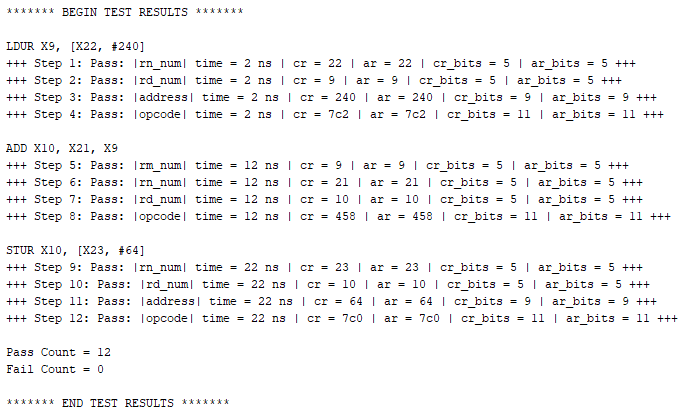
\includegraphics[width=4.75in]{../images/instr_parse_test_output.png}
	\end{center}
\end{figure}

\section{Register File}

Next, we will create the register file.  The register file is a piece of memory in the processor that holds the 32 register values that are used by most instructions (X0-X31).  You will create a new module called regfile (in regfile.v).  The regfile module should retrieve data from the registers on the rising edge of read\_clk as well as write to the registers on the rising edge of write\_clk when the regWrite flag is set.  Two different clocks are used here because the regfile will be read at a different time than it is written to.  The regfile should use a verilog reg array, similar to the array used in instruction memory.  Since we don't currently have the ability to do loads and stores (since we don't have data memory yet), the values for the registers should be stored in a datafile, regData.data and copied into the array during the initial block, just like we did with the instr\_mem.v file.  regData.data is provided for you.  The regfile module will have a lot of similarities to the instr\_mem module, so I recommend reusing concepts and code from the instr\_mem module.

Inputs to the module should include a signal called read\_clk and a signal called write\_clk as well as all inputs shown on the Register file in Figure~\ref{fig:register_file_cutout}.  Don't forget reg\_write.  This is a control signal that determines whether data should be written to the register.  Some instruction write to registers, others do not.  The outputs should be the outputs of the Register file in Figure~\ref{fig:register_file_cutout}.  Use names such as read\_register1, read\_data2, etc.

I have provided the majority of the testbench for this module, regfile\_test.sv.  It  provide input values and verifies that the outputs match expected behavior.  Notice how the testbench utilizes the delay module to create different clocks for read\_clk and write\_clk.  The testbench is designed to test a variety of scenarios and to verify the timing aspects of this module.  Your only job on the testbench is to fill in the correct result (cr) values in the testbench.  They are currently populated with X.

\begin{figure}
	\caption{Instruction Parse and Regfile Diagrams}\label{fig:register_file_cutout}
	\begin{center}
		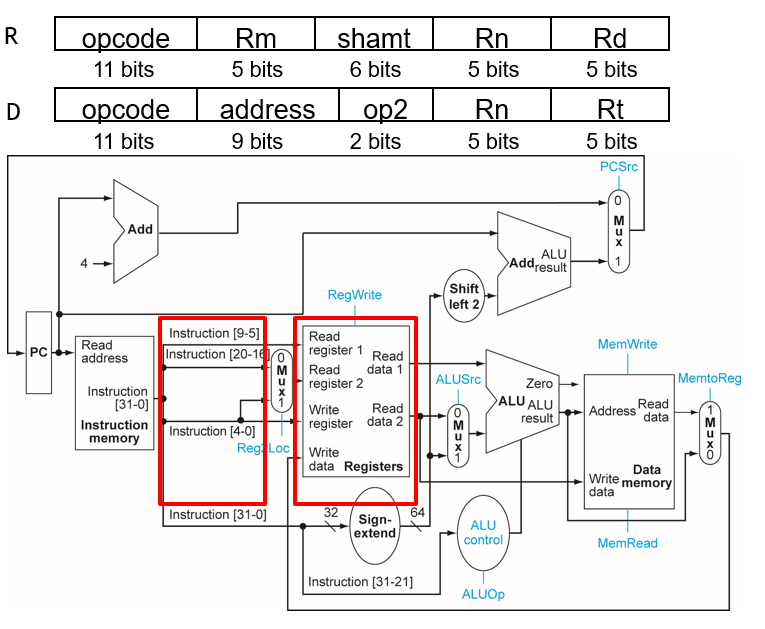
\includegraphics[width=4.75in]{../images/register_file_cutout.png}
	\end{center}
\end{figure} 


\clearpage
\section{Your Assignment}

You are to:
\begin{enumerate}
\item Create an instruction\_parse module as described above.
\item Update instr\_parse\_test and verify the functionality of the instruction\_parse module.  For this testbench, please use hex for instructions and opcodes and unsigned decimal for all other signals.
\item Create a regfile module.
\item Update the regfile\_test module as described above and verify the functionality of the regfile module.  For this testbench, please use signed decimal for all signals.
\item Rather than writing a lab report, please produce a landscape mode PDF file called Lab4\_lastname.pdf that includes (in this order):
\begin{enumerate}
	\item Your name and the lab number.
	\item A snip of the Simulation Results for the instruction\_parse module.  Please show instructions and opcodes in hex and everything else in unsigned decimal.  
	\item A snip of the test results from the Tcl Console for the instruction\_parse module.  This snip should show the entire log from BEGIN TEST RESULTS to END TEST RESULTS.
	\item A snip of the Simulation Results for the regfile module.  Please show everything else in unsigned decimal.  
	\item A snip of the test results from the Tcl Console for the regfile module.  This snip should show the entire log from BEGIN TEST RESULTS to END TEST RESULTS.	
\end{enumerate}
\item Upload Lab4\_lastname.pdf file to Canvas.
\item Zip up your ARM-Lab directory and submit it on Canvas as well.  I will run your code against my correct testbench to verify that your code and testbench work correctly.
\end{enumerate} 